\begin{figure}
\caption{Cost-Push Shock Impulse Responses}\label{fg:irf_cost}
\vspace*{1pc}
\begin{tabular}{ccc}
\multicolumn{3}{c}{Case 1: Rational Expectations}\\
Output Gap & Inflation & Interest Rate \\ 
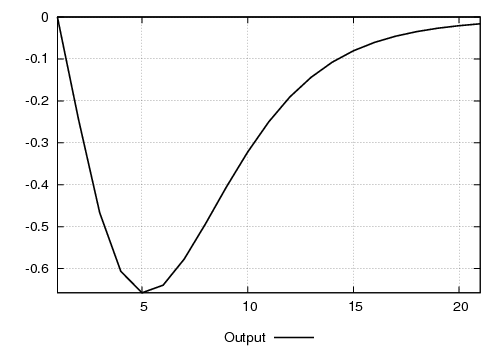
\includegraphics[scale=0.28]{results_re/Output_costshock_irf.png} & 
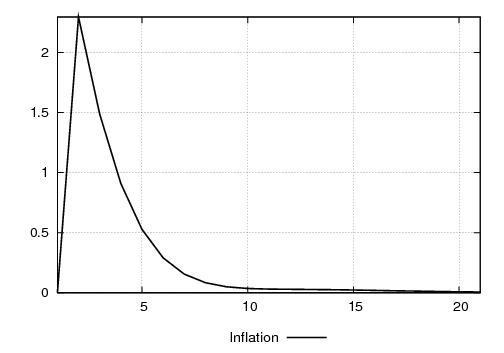
\includegraphics[scale=0.28]{results_re/Inflation_costshock_irf.png} & 
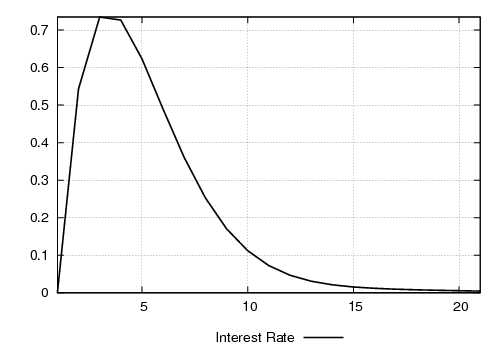
\includegraphics[scale=0.28]{results_re/Interest_Rate_costshock_irf.png} \\ \\ 
\multicolumn{3}{c}{Case 2: Learning with RE Initial Conditions}\\
Output Gap & Inflation & Interest Rate \\ 
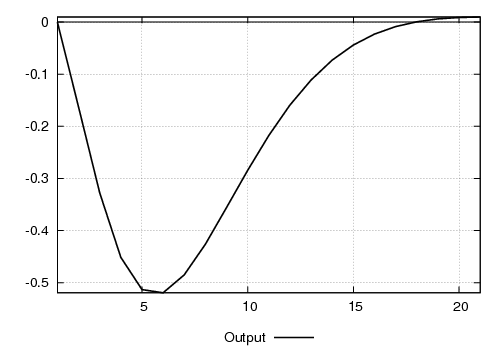
\includegraphics[scale=0.28]{results_reallinit/Output_costshock_irf.png} & 
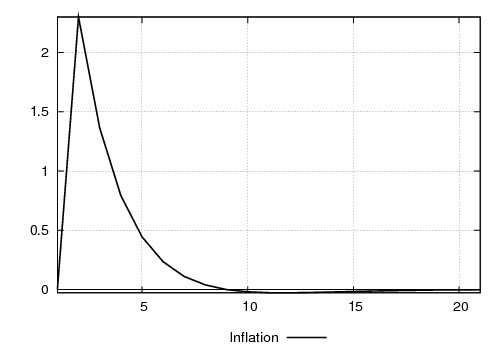
\includegraphics[scale=0.28]{results_reallinit/Inflation_costshock_irf.png} & 
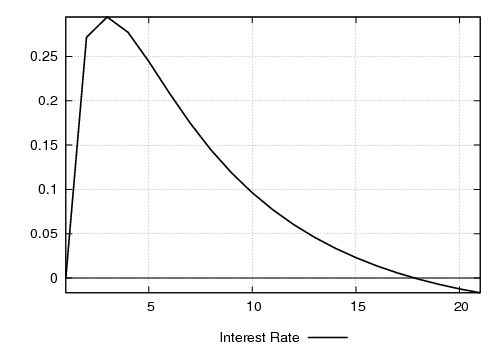
\includegraphics[scale=0.28]{results_reallinit/Interest_Rate_costshock_irf.png} \\ \\ 
\multicolumn{3}{c}{Case 3: Learning with Unobservable Shocks and RE Initial Conditions}\\
Output Gap & Inflation & Interest Rate \\ 
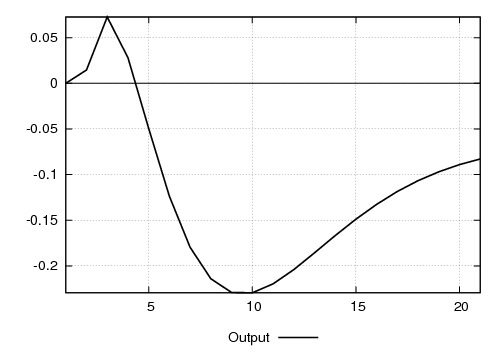
\includegraphics[scale=0.28]{results_reinit/Output_costshock_irf.png} & 
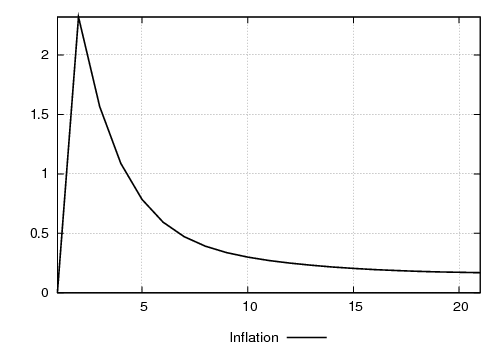
\includegraphics[scale=0.28]{results_reinit/Inflation_costshock_irf.png} & 
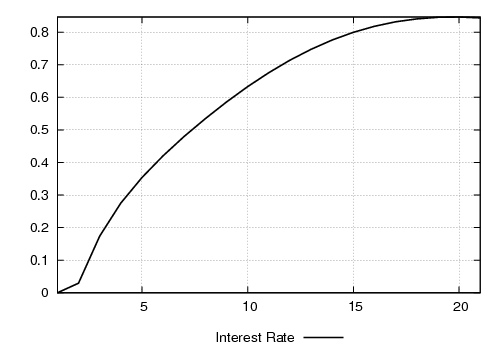
\includegraphics[scale=0.28]{results_reinit/Interest_Rate_costshock_irf.png} \\ \\ 
\multicolumn{3}{c}{Case 4: Learning with Unobservable Shocks and Pre-Sample Initial Conditions}\\
Output Gap & Inflation & Interest Rate \\ 
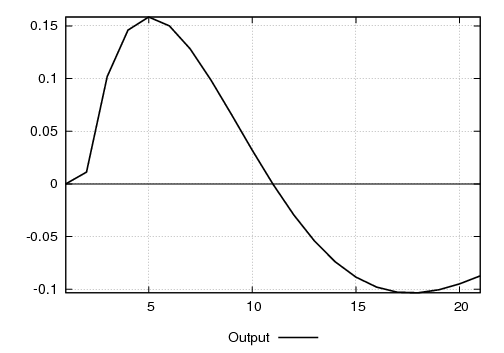
\includegraphics[scale=0.28]{results_wlsinit/Output_costshock_irf.png} & 
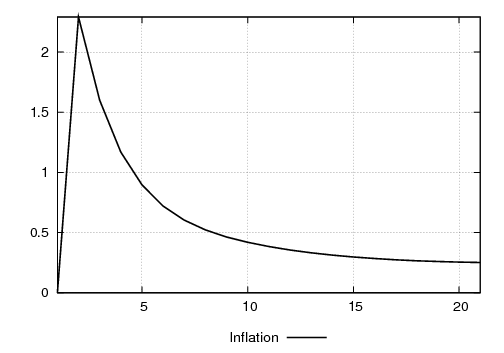
\includegraphics[scale=0.28]{results_wlsinit/Inflation_costshock_irf.png} & 
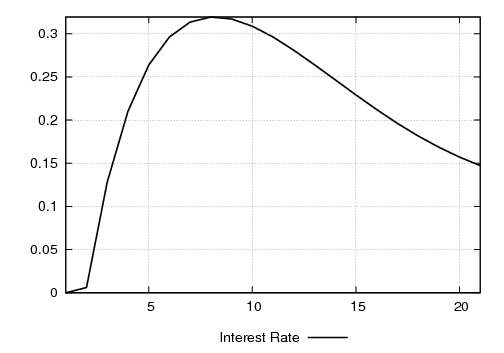
\includegraphics[scale=0.28]{results_wlsinit/Interest_Rate_costshock_irf.png} \\ 
\end{tabular}
\end{figure}
